\documentclass[UTF8]{ctexart} %使用ctex包,中文支持
\usepackage{amsmath}  %数学公式
\usepackage{graphicx} %插图
\usepackage{fancyhdr} %个性化页眉页脚
\usepackage{geometry} %页边距
\usepackage{bm}  % 公式加粗
\usepackage{float} %为了在分栏下插入图片
\usepackage{ulem}  % 换行下划线
%\usepackage{setspace} %行间距
\usepackage{multicol} %用于实现在同一页中实现不同的分栏
\geometry{a4paper,left=2cm,right=2cm,top=2cm,bottom=2cm} % 页边距设置

\title{集成学习笔记}
\author{宋佳欢}
\pagestyle{plain}

\begin{document}
	\maketitle
	\tableofcontents
	\songti \zihao{-4}
	
	\section{Bagging}
		什么情况适合做Bagging:模型容易过拟合(很强的模型),降低模型预测的方差。Bagging并不能帮助模型更好地拟合训练数据。
		\subsection{随机森林}
		决策树在训练数据上很容易达到0错误率(每个叶节点只包含一个样本)。随机森林时决策树的Bagging算法,两种实现方式:
		
		1.在m个样本的数据集D中,有放回地随机采样m个样本,将其拷贝进$D_1$。$D_1$中会有重复的样本,且部分D中的样本没有在$D_1$中出现。重复上述过程,得到n个不同的数据集${D_1,D_2,\cdots,D_n}$,用这些数据集分别训练n个决策树,构成随机森林。
		
		2.随机地限制某些特征在生成决策树时禁用,这样也能得到若干不同的决策树。
		
		out-of-bag validation for Bagging:
		若方法1训练决策树,可将那些在训练集中没有出现过的那些样本用于测试,这样就可以不用划分训练集和测试集了。
	\section{Boosting}
		什么情况适合做boosting:想要提升弱分类器的分类性能
		\begin{figure}[H]
			\centering{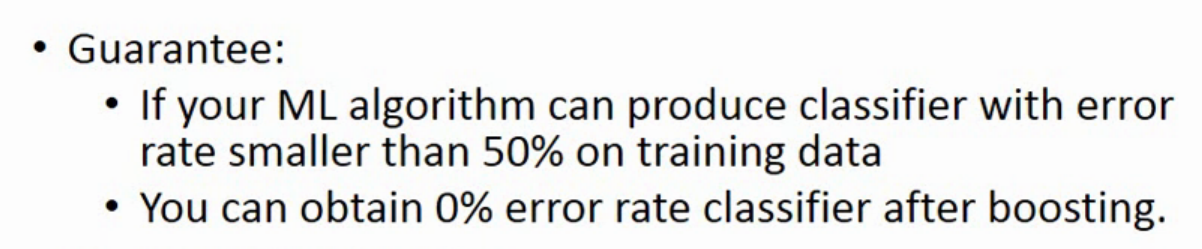
\includegraphics[scale=0.3]{1.png}}
		\end{figure}
		\subsection{Boosting的框架}
		
			1.得到一个弱分类器$f_1(x)$。
			
			2.找到另一个分类器$f_2(x)$取帮助$f_1(x)$。但是两者不能太相似,最好是互补的。
				
			3.同理,再找到另一个分类器$f_3(x)$取帮助$f_2(x)$。
			
			$\cdots$,最后结合所有的分类器。
			每个分类器都是按顺序学习的。
			
			为了获取不同的分类器,在不同的数据集上训练。为了得到不同的训练集,可以重采样来制造多个数据集;也可以为每个样本设置不同的权重,在实现中,只需在损失函数前为每个样本乘上一个权重即可:
			\[L(f)\sum_nl(f(x^n,\hat{y}^n))\Longrightarrow L(f)\sum_nu^nl(f(x^n,\hat{y}^n))\]
			其中$u^n$即为每个样本的权重。
		\subsection{Adaboost}
			主要思想:使用分类器$f_1(x)$分类失败的那些样本取训练$f_2(x)$。
			
			定义$f_1(x)$在训练集上的错误率为$\varepsilon_1$
			\[\varepsilon_1 = \frac{\sum_nu_1^n\delta(f_1(x^n)\neq\hat{y}^n)}{Z_1}, \quad Z_1=\sum_nu_1^n\]
			$u_1^n$为训练第一个分类器时的第n个样本的权重。$\delta$函数括号内成立时等于1,否则等于0。若弱分类器由于随机分类,则有错误率$\varepsilon_1<0.5$。
			
			根据$u_1^n$调整$u_2^n$,即增大$f_1(x)$分类错误的样本的权重,减小分类正确的样本的权重,使得在训练$f_2(x)$时,分类器更加侧重于$f_1(x)$分类错误的样本的权重,使得两个分类器互相互补。调整权重使得$u_2^n$满足:
			\[\frac{\sum_nu_2^n\delta(f_1(x^n)\neq\hat{y}^n)}{Z_2}=0.5, \quad Z_2=\sum_nu_2^n\]
			\begin{figure}[H]
				\centering{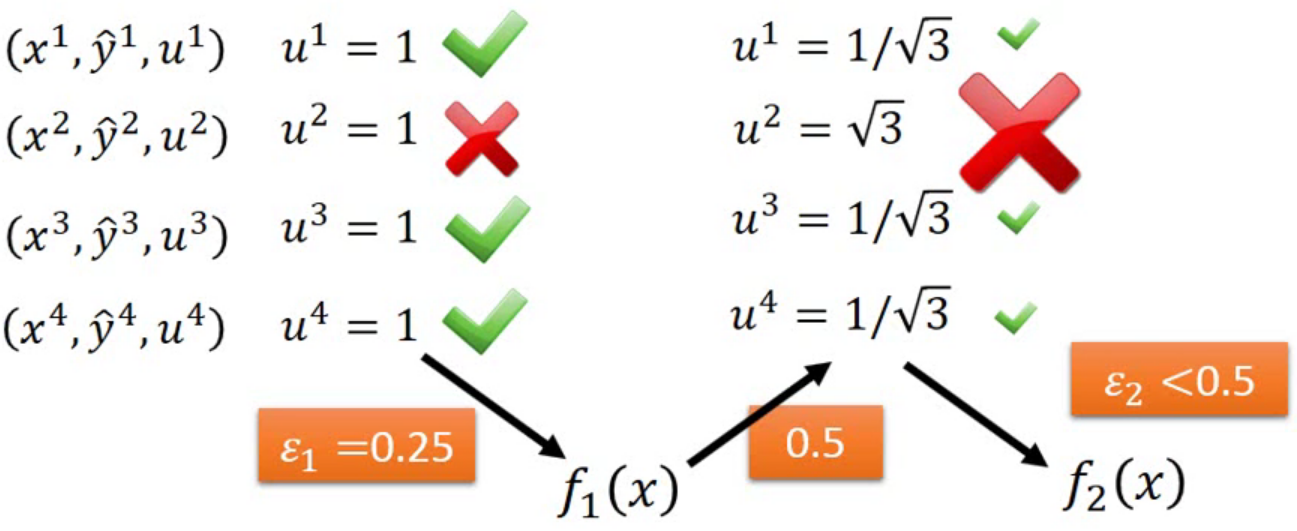
\includegraphics[scale=0.3]{2.png}}
			\end{figure}
			
			\textbf{如何更改权重?}
			
			\quad1.如果样本$x^n$被$f_1$分类错误,则$u_2^n=u_1^n\times d_1,\quad d_1>1$,增加权重。
			
			\quad2.如果样本$x^n$被$f_1$分类正确,则$u_2^n=u_1^n/d_1,\quad d_1>1$,减小权重。
			
			接下来的问题是如何求解$d_1$。我们将$u_2^n$用$u_1^n$和$d_1$代掉,可得:
			\begin{figure}[H]
				\centering{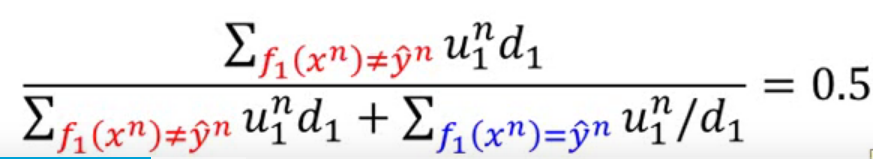
\includegraphics[scale=0.3]{3.png}}
			\end{figure}
			将上式取倒数:
			\begin{figure}[H]
				\centering{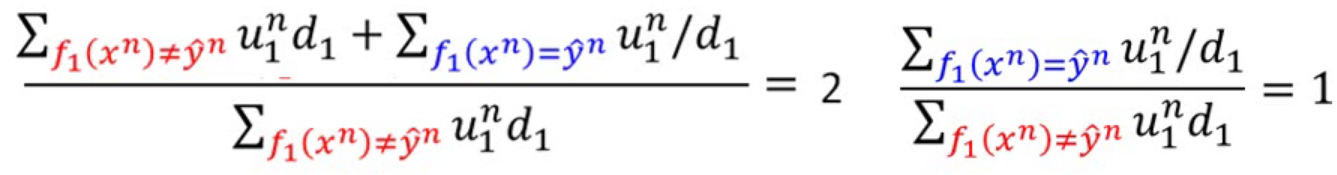
\includegraphics[scale=0.3]{4.png}}
			\end{figure}
			即:
			\begin{figure}[H]
				\centering{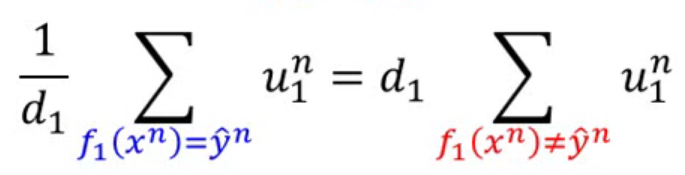
\includegraphics[scale=0.25]{5.png}}
			\end{figure}
			因为:
			\begin{figure}[H]
				\centering{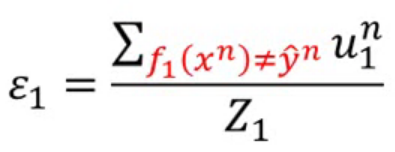
\includegraphics[scale=0.3]{6.png}}
			\end{figure}
			所以等式变为:
			\[Z_1(1-\varepsilon_1)/d_1 = Z_1\varepsilon_1d_1\]
			得$d_1=\sqrt{(1-\varepsilon_1)/\varepsilon_1}$
			
			\begin{figure}[H]
				\centering{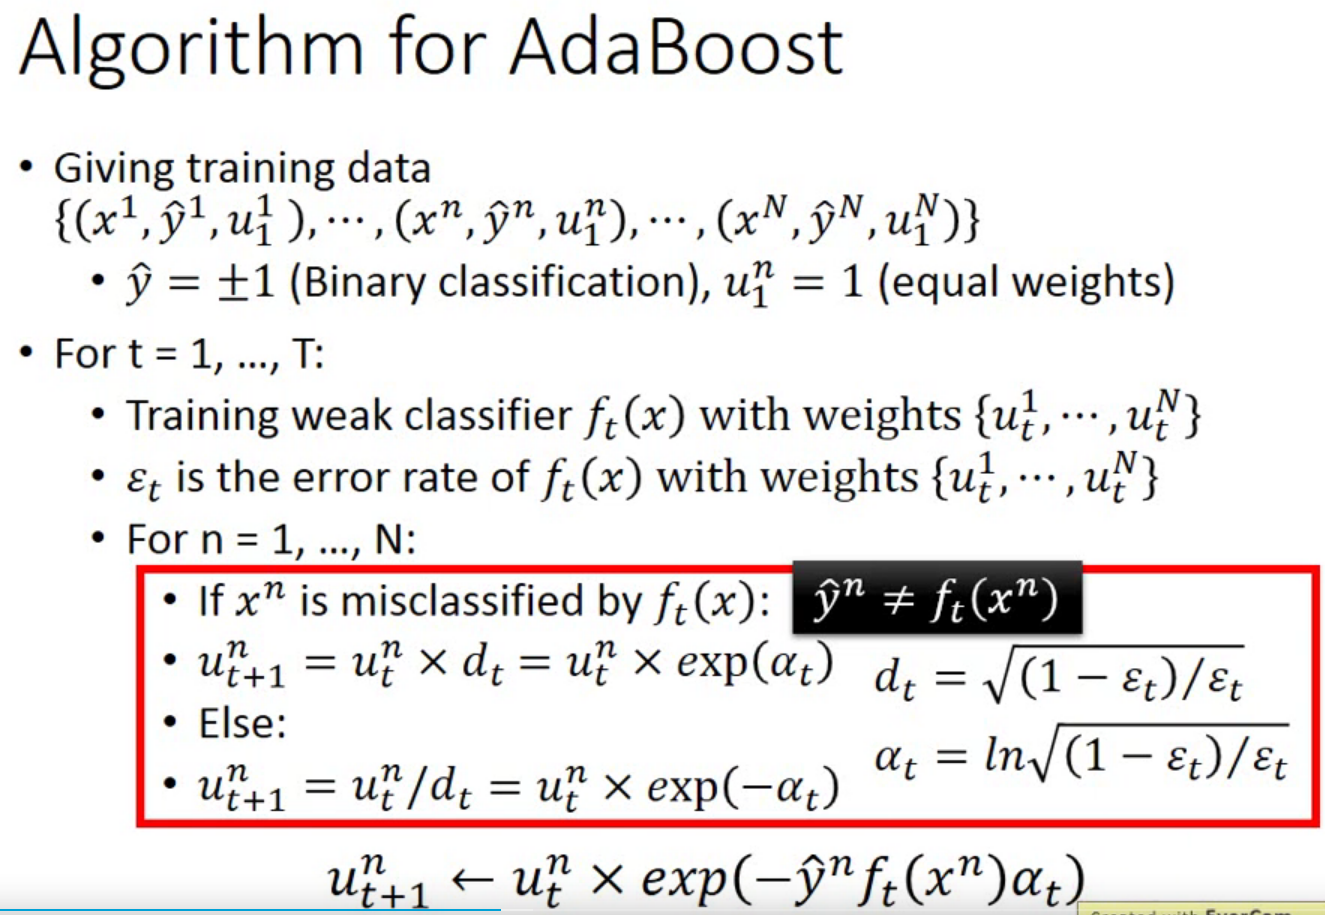
\includegraphics[scale=0.3]{7.png}}
			\end{figure}
			上述算法流程中,为了将红框权重的更新整合到一个式子里,对$d_t$取对数得到$\alpha_t$,再在其正负号上做文章。
			
			最后,得到一系列分类器${f_1(x),f_2(x),\cdots, f_t(x),f_T(x)}$,\textbf{如何将他们集合起来?}
			
			\quad 1.统一的权重,将输出相加,取正负,$H(x)=sign(\sum_{t=1}^Tf_t(x))$
			
			\quad 2.每个分类器分配不同的权重,$H(x)=sign(\sum_{t=1}^T\alpha_tf_t(x))$。因为$\alpha_t=ln\sqrt{(1-\varepsilon_t)/\varepsilon_t}$,如果分类器的训练错误率$\varepsilon_t$越小,则权重$\alpha_t$会越大,即越好的分类器权重越大 。下图显示的权重$\alpha_t$与训练错误率$\varepsilon_t$的关系。
			\begin{figure}[H]
				\centering{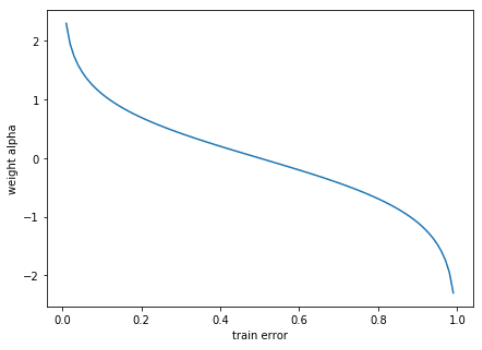
\includegraphics[scale=0.6]{15.png}}
			\end{figure}
			
			\textbf{例子:}
			\begin{figure}[H]
				\centering{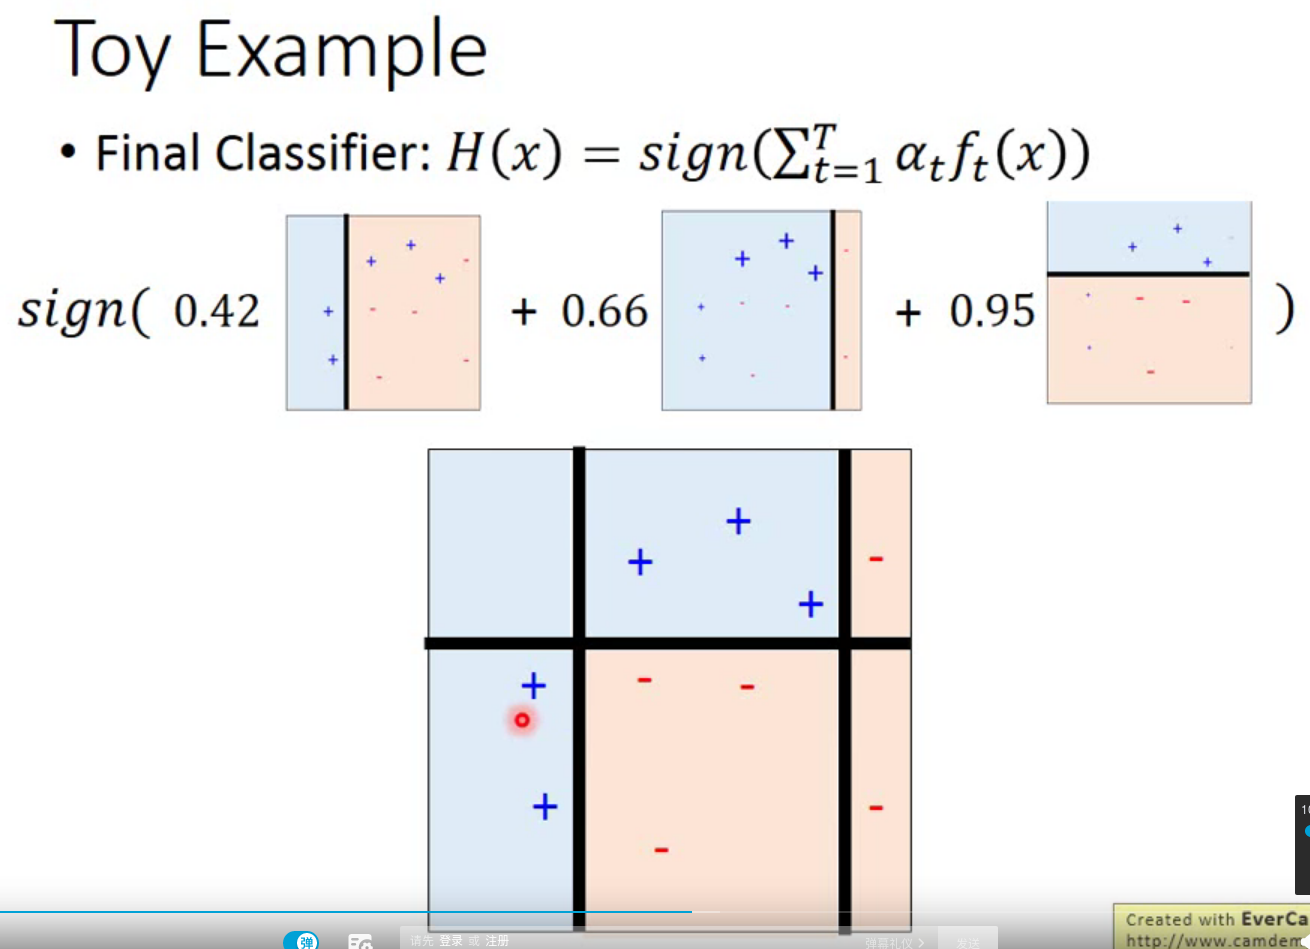
\includegraphics[scale=0.3]{8.png}}
			\end{figure}
		\subsection{Adaboost数学证明}
			最终分类器:
			\[H(x) = sign(\sum_{t=1}^T\alpha_tf_t(x))\]	
			令$\sum_{t=1}^T\alpha_tf_t(x) = g(x)$。
			
			证明Adaboost算法能够减小训练数据的错误率,训练错误率=
			\[\frac{1}{N}\sum_n\delta(H(x^n)\neq\hat{y}^n) = \frac{1}{N}\sum_n\delta(\hat{y}^ng(x^n)<0)\leq
			\frac{1}{N}\sum_nexp(-\hat{y}^ng(x^n))\]
			训练错误率有上界,只需证明该上界在训练过程中逐渐减小,则可证明训练错误率也在减小。
			\begin{figure}[H]
				\centering{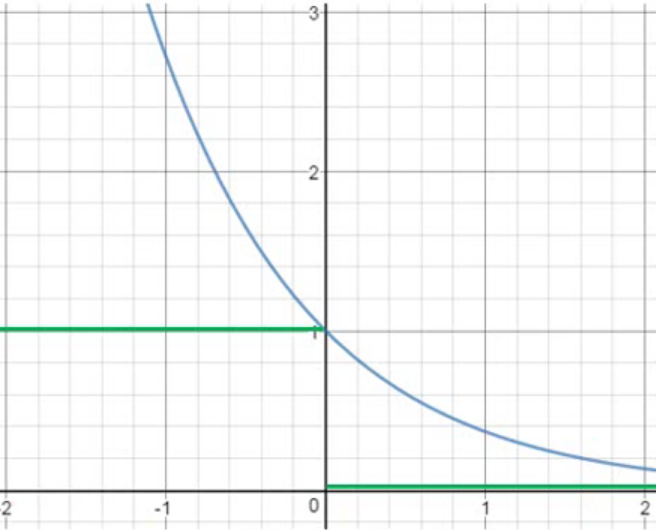
\includegraphics[scale=0.4]{9.png}}
				\caption{绿色为$\delta(\hat{y}^ng(x^n)<0)$,蓝色为$exp(-\hat{y}^ng(x^n))$ }
			\end{figure}
			
			证明:
			
			$Z_t$是在训练$f_t$时,所有的权重之和。所以$Z_{T+1} = \sum_nu_{T+1}^n$。
			因为:
			\[u_1^n=1,\quad u_{t+1}^n=u_t^n\times exp(-\hat{y}^nf_t(x^n)\alpha_t)\]
			
			所以:
			\[u_{T+1}^n = \prod_{t=1}^Texp(-\hat{y}^nf_t(x^n)\alpha_t)\]
			
			所以:
			\[Z_{T+1} = \sum_n\prod_{t=1}^Texp(-\hat{y}^nf_t(x^n)\alpha_t)
			=\sum_nexp\Big(-\hat{y}^n\sum_{t=1}^Tf_t(x^n)\alpha_t\Big)\]
			
			即:
			\[Z_{T+1} = \sum_nexp(-\hat{y}^ng(x^n))\]
			
			所以训练错误率:
			\[\frac{1}{N}\sum_n\delta(\hat{y}^ng(x^n)<0)\leq\frac{1}{N}\sum_nexp(-\hat{y}^ng(x^n))=\frac{1}{N}Z_{T+1}\]
			
			证明每轮训练的权重之和$Z_t$递减,原命题即可得证。
			$Z_t$与上一个$Z_{t-1}$之间的关系如下,按错误率的比例增大或减小:
			\[\begin{aligned}
			Z_t = Z_{t-1}\varepsilon_texp(\alpha_t)+Z_{t-1}(1-\varepsilon_t)exp(-\alpha_t)\\
			=Z_{t-1}\varepsilon_t\sqrt{(1-\varepsilon_t)/\varepsilon_t}+ Z_{t-1}(1-\varepsilon_t)\sqrt{\varepsilon_t/(1-\varepsilon_t)}\\
			=Z_(t-1)\times2\sqrt{\varepsilon_t(1-\varepsilon_t)}
			\end{aligned}\]
			
			因为$\varepsilon_t< 0.5$,所以$2\sqrt{\varepsilon_t/(1-\varepsilon_t)} < 1$,可得:
			\[Z_{T+1} = N\prod_{t=1}^T2\sqrt{\varepsilon_t/(1-\varepsilon_t)}\]
			因此每一轮训练都可以使得训练误差会越来越小。
			
		\subsection{Gradient Boosting}
			在实现Adaboost的过程中会出现下图的情况,虽然随着横轴训练数量和分类器数量的增加,训练数据的错误率很快达到0,但是测试数据的错误率并没有收敛。原因是虽然训练数据全部都能被正确识别,看似分类器以及没有什么东西可以学了,但是分类器的间隔在一开始是很小的,在后器随着分类间隔的增大,测试数据的错误率才会下降。
			\begin{figure}[H]
				\centering{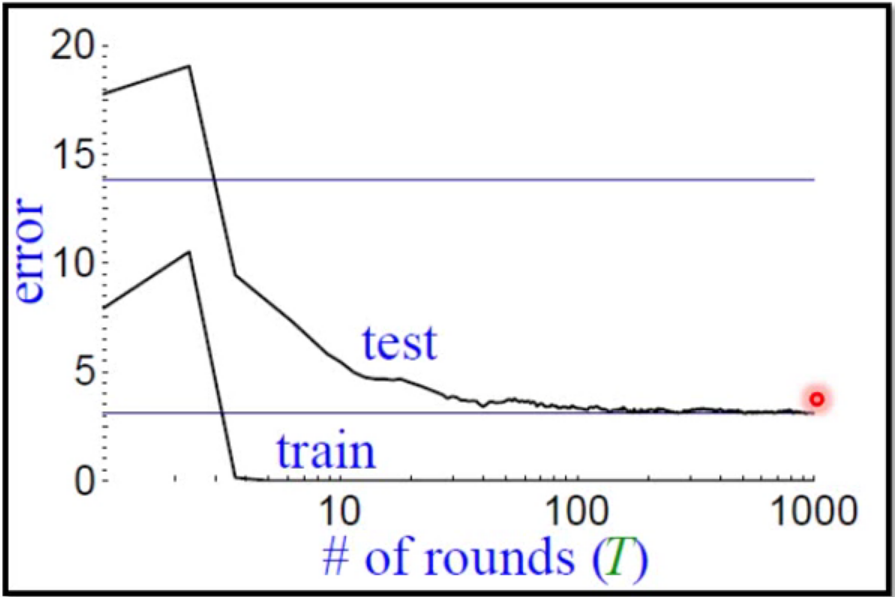
\includegraphics[scale=0.3]{10.png}}
			\end{figure}
			
			最终的分类器:
			\[H(x) = sign(\sum_{t=1}^T\alpha_tf_t(x)),\quad\sum_{t=1}^T\alpha_tf_t(x) = g(x)\]	
			
			令:
			\[Margin=\hat{y}g(x)\]
			
			可以看出,Margin越大,模型的容错能力就越大。在Adaboost的实现过程中,我们可以将训练数据的错误率的上界看做目标函数,我们的目标实际上是在最小化目标函数,下图比较了其他两种分类器的损失函数。在训练过程中,损失函数会不断地减小,增大分类间隔,提高分类器的鲁棒性。
			\begin{figure}[H]
				\centering{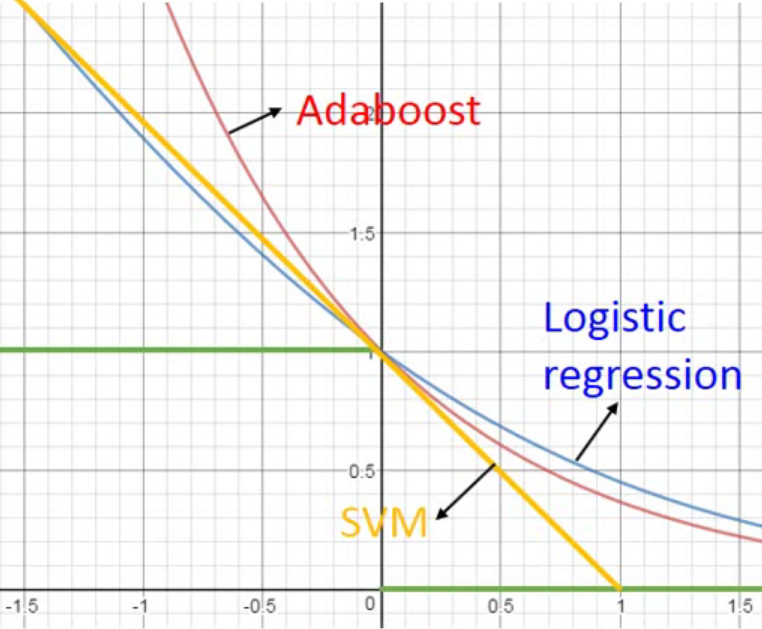
\includegraphics[scale=0.3]{11.png}}
			\end{figure}
			
			若将损失函数定义为:
			\[L(g) = \sum_nexp(-\hat{y}g(x^n))\]
			这个损失函数是合理的,如果分类正确,$\hat{y}$和$g(x^n)$是同号的。从Gradient Boosting和Adaboost两个角度来看,下一个增加的弱分类器的方向应该要和梯度下降的方向相同.
			\begin{figure}[H]
				\centering{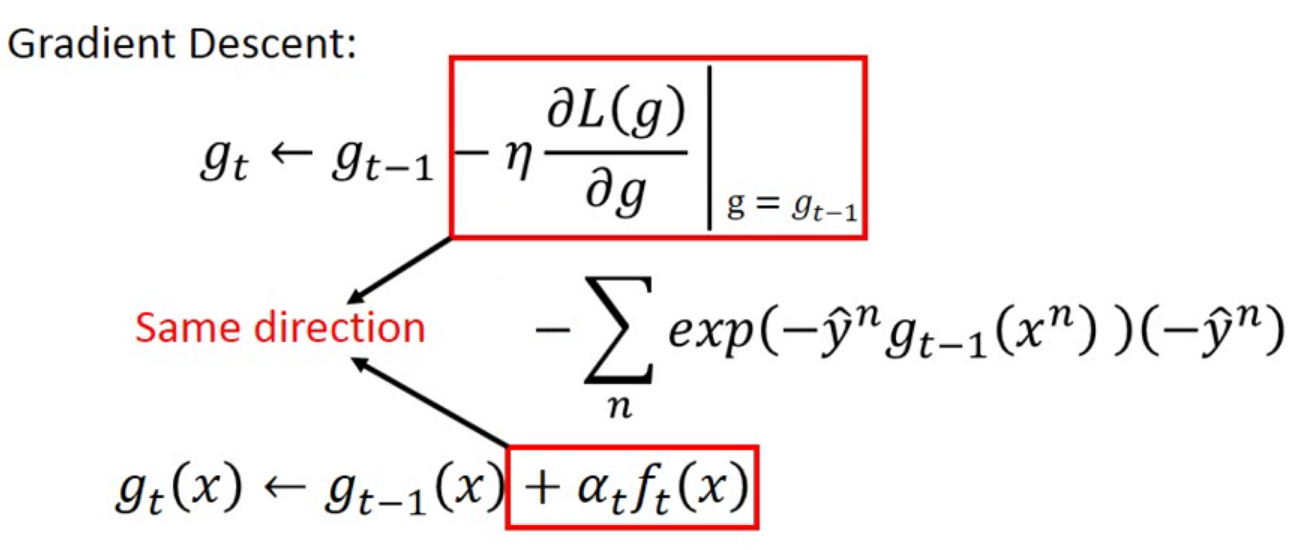
\includegraphics[scale=0.25]{12.png}}
			\end{figure}
			
			因为同向,将$f_t(x)$与梯度相乘,并使之最大化,它的权重与Adaboost中的相同,Adaboost是Gradient Boosting中取了某个特定的损失函数的一种特例。Gradient Boosting可以定义不同的损失函数。
			\begin{figure}[H]
				\centering{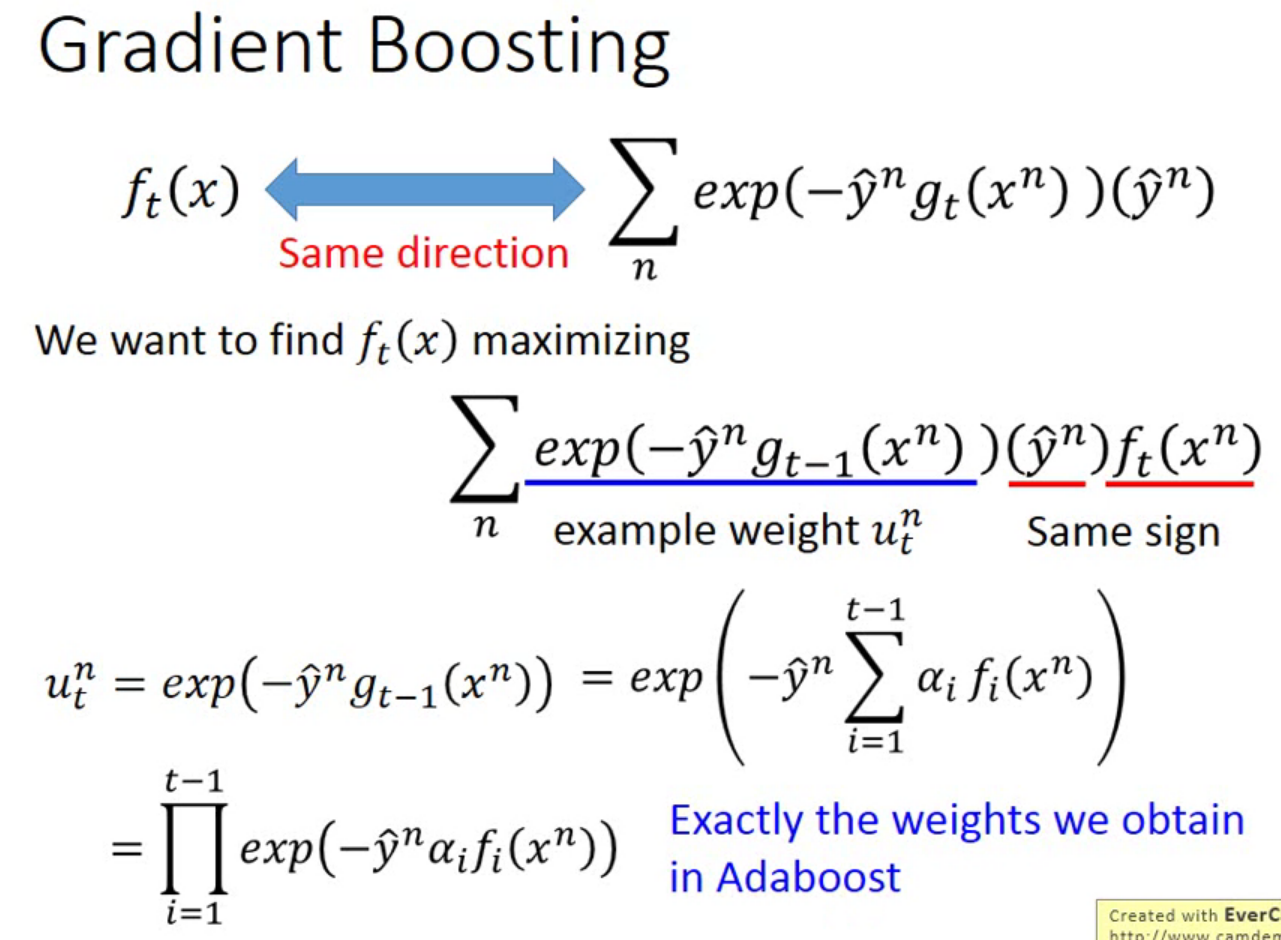
\includegraphics[scale=0.27]{13.png}}
			\end{figure}
			
			\begin{figure}[H]
				\centering{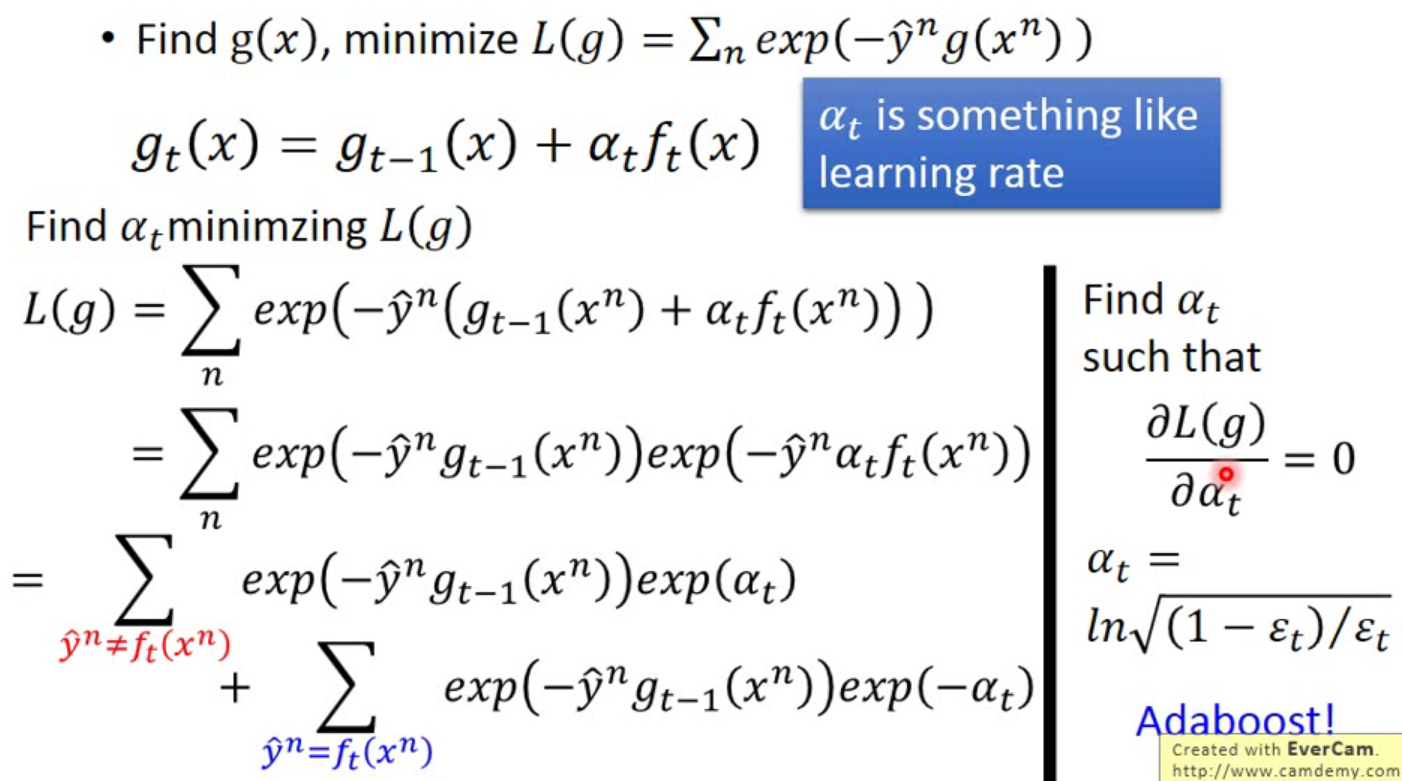
\includegraphics[scale=0.27]{14.png}}
			\end{figure}
			
			
\end{document}